\documentclass[a4paper,english]{article}
\usepackage[utf8]{inputenc}
\usepackage[russian, english]{babel}
\usepackage{natbib}
\usepackage{graphicx, float}
\usepackage{listings}
\usepackage{xcolor}
\usepackage{pgfplots}
\lstset { %
    language=C++,
    backgroundcolor=\color{blue!5}, % set backgroundcolor
    basicstyle=\footnotesize,% basic font setting
}

\title{Пресмятане на Pi – Ramanujan}
\author{Янислав Василев}
\date{Юни 2019}





\begin{document}

\begin{figure}
\centering

\includegraphics[scale=0.5]{..\assets\su.jpg}
\end{figure}

\maketitle
\newpage
\section{Увод в проекта}
Проектът реализира паралелен алгоритъм за намирането на \begin{math}\frac{1}{\pi}\end{math} по формулата на Ramanujan:
\[
    \frac{2\sqrt{2}}{9801}\sum_{k=0}^{\infty} \frac{(4k!)(1103 + 26390k)}{k!^4 396^(4k)}
\]

Ако разгледаме формулата внимателно забялзваме, че всеки един наш член на редицата, се нуждае от пресмятането на \begin{math}k!\end{math} и \begin{math}4k!\end{math}, това означава, че ние може да преизползваме вече пресметнатите от предходни калкулации факториели с цел да олекотим работата на алгоритъма това е също така в основата на кеширането на нашият алгоритъм.\hfill

\vspace{3mm}

Програмата удволетворява следните функционални изисквания:

\begin{itemize}
    \item Команден параметър задаващ точността на пресмятанията 
    
    \begin{center}
    \textit {\texttt{-{}-}i=23572 или \texttt{-{}-}iterations=23572}
    \end{center}
    
    това, ще зададе на програмата да пресметне 23572 члена от сумата на Ramanujan, също така прецизността на решението автоматично ще бъде настроена на \begin{math}23572 * 8\end{math} тъй, като всеки един член на сумата добавя 8 нови знака към \begin{math}\frac{1}{\pi}\end{math}. Този параметър е задължителен.
    \item Команден параметър, който задава максималния брой нишки (задачи) на които разделяме работата по пресмятането на \begin{math}\frac{1}{\pi}\end{math}
    
    \begin{center}
        \textit{\texttt{-{}-}t=1 или \texttt{–{}-}threads=1}
    \end{center} 
    
    това, ще зададе на програмата възможност да работи с една нишка. За максимален ефект се препоръчва броят на логическите ядра на процесорът, на които програмата ще се изпълнява. В случай, че този параметър липсва, програмата ще се изпълни серийно (т.е с една нишка). Този параметър не е задължителен.
    \item Команден параметър, чрез който програмата извежда подходящи съобщения на различните етапи от работата си, както и времето отделено за изчисление и резултата от изчислението 
    
    \begin{center}
        \textit{\texttt{-{}-}verbosity=quiet или \texttt{-{}-}verbosity=verbose}
    \end{center}
    
    В първият случай програмата ще регистрира само минималният покриващ изискванията набор от съобщения (с какви аргументи е стартирана програмата, колко време е отнело пресмятането и резултата), а във вторият случай има по-подробна информация като това колко време е отнело на една нишка да приключи своята работа и д.р. В случай, че този параметър липсва програмата ще назначи служебно такъв. Този параметър не е задължителен.
    \item  Команден параметър, чрез който се указва в кой изходен файл да бъде изписан разултата и контролните съобщения. 
    
    \begin{center}
        \textit{\texttt{-{}-}o=result.txt или \texttt{-{}-}output =result.txt}
    \end{center}
    
    В случай, че този параметър липсва програмата ще назначи автоматично служебно име за файла. Този параметър не е задължителен.
    
    \item Команден параметър, чрез който се избира оптимизирана (не наивна) стратегия по разпределяне на работата по нишките.
    
    \begin{center}
        \textit{\texttt{-{}-}optimized}
    \end{center}
    
    В случай, че този параметър не е посочен, програмата ще избере наивно разделяне на работата по работещите нишки. Подразбира се, че ако сме посочили този параметър и това програмата да се изпълнява серийно, то този параметър няма ефект.
    
    \item Помощен команден параметър,
    
    \begin{center}
        \textit{\texttt{-{}-}h или \texttt{-{}-}help}
    \end{center}
    
    който изписва на екрана всички опции(командни параметри) на програмата, техните свойства, стойности по подразбиране и функции.
\end{itemize}


\section{Проектиране и реализация}
    Алгоритъмът е реализиран на C++11 на платформа Windows с Microsoft Visual C++ компилатор, като е изпозван модела за паралелизъм по данни или Single Program-Multiple Data(SPMD) като нишките работят асинхронно една от друга.\hfill
    Архитектурата на програмата е по модела Master-Slave, тоест имаме една основна нишка (наречена още main) чакаща всички останали да свършат своята работа.\hfill
    Един начин да се стартира програмата след като тя е компилиране е например:
    \begin{center}
        \textit{main.exe \texttt{-{}-}iterations=100 \texttt{-{}-}threads=8}
    \end{center}
    ще стартира програмата с осем нишки за пресмятането на сто члена от формулата.\hfill
    Още при пускането на програмата всички командни параметри се запазват в обект от тип \lstinline{ProgramOptions}, който след това се ползва да настройването на \lstinline{Logger::options}, прецизността на типа, който ползва програмата за пресмятане на \(\frac{1}{\pi}\) (\lstinline{boost::multiprecision::mpfr_float}) и за разпределянето на работата по нишките, чийто задача има \lstinline{SeparationStrategy} обектът.\hfill
    Програмата има два вида стратегии на разпределяне на работа.
    
        \begin{itemize}
        \item Наивен\hfill
        
        \vspace{3mm}
            Този вид разпределение е най-базовото и с нарастване на броят итерации поискани от потребителя започва да създава проблеми. Това, което прави е например ако имаме да решим 1000 итерации с 5 нишки, той разделя работата по равно на всяка нишка. Така работата ще за всяка една от тях ще изглежда така\hfill
            \begin{center}
                \textit{1 : [0, 250], 2: [251, 500], 3: [501, 750], 4: [751, 1000],}
            \end{center}
            където 1-5 са идентификатори на нишките а [x,y] е интервалът, в който нишката ще работи.\hfill
            
            На пръв поглед това изглежда като добро решение, но малко по-подробен анализ показва, че работата на нишка 4 в нашият пример е много по-тежка от работата на нишка 1, което води до неоптимални резултати.\hfill
            
            Алгоритъмът, който го имплементира
            \begin{lstlisting}
simple_ranges
NaiveSeparationStrategy::Separate(long iterations,
short threads)
{
	simple_ranges ranges;
	if (threads == 0)
		return ranges;

	ranges.reserve(threads);

	auto chunk = iterations / threads;
	auto remainder = iterations % threads;

	auto loopIterations = 0;
	for (auto partition = 0; 
	    partition <= iterations - chunk + loopIterations; 
	    partition += chunk + 1)
	{
		ranges
		.emplace_back(partition, 
		              partition + chunk > iterations ?
		              iterations : partition + chunk);
		++loopIterations;
	}

	return ranges;
}
            \end{lstlisting}
            
        \item Оптимизиран\hfill
        
        \vspace{3mm}
            За разлика от наивният вид на разпределение, този няма такъв проблем. Ако вземем предишното ни тестово изпълнение, където с пет нишки трябва да пресметнем хиляда члена от сумата, този път нашето разпределени ще изглежда по този начин
            \begin{center}
                \textit{1:[0,100]\(\cup\)[900,1000], 2:[101,200]\(\cup\)[800,899], 3:[201,300]\(\cup\)[700,799], 4:[301,400]\(\cup\)[600,699], 5:[401,500]\(\cup\)[500,599]}
            \end{center}
            Вижда се, че сега работата наистина е не само по разпределена по равно, но и по сложност.\hfill
            
            Алгоритъмът, реализиращ това разпределение
            \begin{lstlisting}
advanced_ranges
OptimizedSeparationStrategy::Separate(long iterations, 
short threads)
{
	advanced_ranges ranges;
	if (threads == 0)
		return ranges;

	ranges.reserve(threads);

	auto leftChunk = 0, rightChunk = 0;
	
	if ((iterations / threads) % 2 != 0)
	{
		leftChunk = (iterations / threads) / 2;
		rightChunk = (iterations / threads) / 2 + 1;
	}
	else
	{
		leftChunk = rightChunk
		          = (iterations / threads) / 2;
	}

	long l = 0, 
	     r = iterations, 
	     previous_l = l, previous_r = r;

	while (l < r)
	{
		ranges
		.emplace_back(
		   std::make_pair(previous_l, l + leftChunk),
		   std::make_pair(r - rightChunk, previous_r)
		);

		previous_l = l + leftChunk + 1;
		previous_r = r - rightChunk - 1;

		l += leftChunk;
		r -= rightChunk;
	}

	// make last range excluding last number
	// as it will be calculated from the 
	// second last range.
	ranges.back().first.second--;

	return ranges;
}
            \end{lstlisting}
            
        \end{itemize}
        
        След избирането на стратегия същинската работа започва.
        Основната нишка (main <-> master) има за цел да изчака всички работещи (workers <-> slaves) и след това да запише резултата.
\section{Тестване}
    Програмата е тествана на тестовият сървър rmi.yacht.net.
    
    Следната таблица е построена от резултатите при пресмятане на 10 000 члена от сумата при следните опции
    \begin{center}
        \textit{\texttt{-{}-}iterations=10000 \texttt{-{}-}threads=X (\texttt{-{}-}optimized)}
    \end{center}

% Preamble: \pgfplotsset{width=10cm,compat=1.15}
\begin{tikzpicture}
\begin{axis}
[
    xtick=data,
    xlabel=Threads,
    ylabel=Time(ms),
    enlargelimits=0.15,
    enlarge x limits={0.15},
    tick label style={font=\footnotesize},
    legend style={
        at={(0.5,-0.20)},
        anchor=north,
        legend columns=-1
    },
    ybar=1pt,
    symbolic x coords={1,2,3,4,5,6,7,8,12,16,24,32},
    bar width=5pt,
]
\addplot coordinates {
(1,22.77) (2,8.3) (3,5.45) (4,3.95) 
(5,3.13)  (6,2.55) (7,2.44) (8, 2.11)
(12,1.77) (16,1.50) (24,1.18) (32,1.03)
};
\addplot coordinates {
(1,22.77) (2,10.18) (3,7.13) (4,4.92) 
(5,3.9) (6,3.21) (7,2.82) (8, 2.41)
(12,2.07) (16,1.64) (24,1.24) (32,1.01)
};

\legend{Optimized,Naive}
\end{axis}
\end{tikzpicture}
\vspace{15mm}
\newline
    програмата е компилирана с компилатор g++ с опция -О3 за максимално бързодействие.
    
    Ускорението, което се получава от предишната таблица.
    
\begin{figure}[H]
    \hspace*{-2cm}
    \centering
    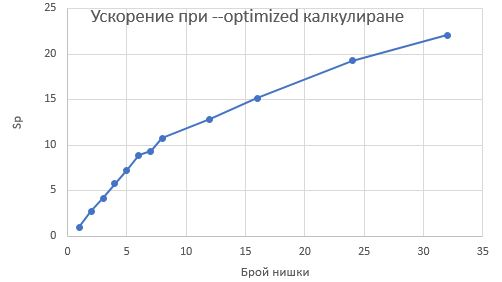
\includegraphics{..\assets\Sp.JPG}
\end{figure}
\newpage
    Ефикасността, която се получава.
    
\begin{figure}[H]
    \centering
    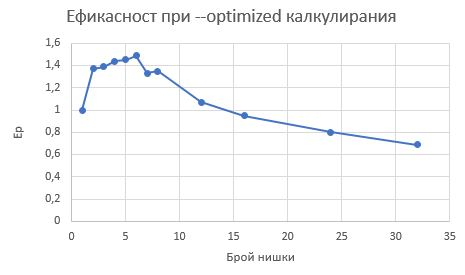
\includegraphics{..\assets\Ep.JPG}
\end{figure}

    
    
\textbf{T1} – времето за изпълнение на серийната програма (използваща една нишка). \newline
    \textbf{Tp} – времето за изпълнение на паралелната програма, използваща p нишки. \newline
    \textbf{Sp = T1/Tp} – ускорението, което програмата има при използването на p нишки. \newline
    \textbf{Ep = Sp/p} – ефективността (ефикасността) на програмата при използването на p нишки.

\end{document}
